\section*{Results}
The empirical AUC target was achieved. Table~\ref{tab:model-comparison} shows the model comparison. TF-IDF logistic regression was selected by validation ROC AUC, with validation ROC AUC 0.977, Brier score 0.054, and expected calibration error 0.012. On the internal test split, the same model achieved ROC AUC 0.976 (95\% bootstrap CI 0.975 to 0.977), PR AUC 0.967, accuracy 0.926, F1 0.916, sensitivity 0.935, specificity 0.918, Brier score 0.055, and expected calibration error 0.011. The internal-test confusion matrix for the selected threshold contained 12,681 true positives, 16,266 true negatives, 1,448 false positives, and 875 false negatives.

\begin{table}[!ht]
\centering
\caption{\textbf{Model comparison on validation and internal test splits.} Model selection used validation ROC AUC, with Brier score as a secondary calibration criterion.}
\small
\begin{tabular}{lrrrrrr}
\hline
Model & Val AUC & Test AUC & Test PR AUC & Test F1 & Test Brier & Test ECE \\
\hline
bilstm & 0.975 & 0.974 & 0.965 & 0.908 & 0.060 & 0.010 \\
bilstm\_dropout & 0.965 & 0.964 & 0.953 & 0.893 & 0.071 & 0.015 \\
ffnn\_avg\_embeddings & 0.962 & 0.962 & 0.948 & 0.887 & 0.074 & 0.010 \\
lstm & 0.892 & 0.891 & 0.886 & 0.800 & 0.129 & 0.039 \\
majority\_baseline & 0.500 & 0.500 & 0.434 & 0.000 & 0.246 & 0.002 \\
tfidf\_linear\_svm & 0.976 & 0.974 & 0.964 & 0.915 & 0.057 & 0.011 \\
tfidf\_logistic\_regression & 0.977 & 0.976 & 0.967 & 0.916 & 0.055 & 0.011 \\
\hline
\end{tabular}
\begin{flushleft}\footnotesize All values are from saved run metrics. Classical models used validation-fitted Platt calibration; neural models used validation-fitted temperature scaling.\end{flushleft}
\label{tab:model-comparison}
\end{table}


The strongest neural model was the BiLSTM, with internal test ROC AUC 0.974, compared with 0.976 for TF-IDF logistic regression and 0.974 for TF-IDF linear SVM. The unidirectional LSTM was weaker, with internal test ROC AUC 0.891. This pattern indicates that lightweight recurrence did not provide a clear advantage over sparse lexical baselines under the CPU-feasible protocol.

Table~\ref{tab:calibration} reports calibrated probability metrics. The selected model's internal calibration was strong by the saved metrics, with internal-test Brier score 0.055, expected calibration error 0.011, calibration intercept -0.021, and calibration slope 0.983. External calibration was weaker, with Brier score 0.085, expected calibration error 0.024, and calibration slope 0.770, consistent with corpus and label shift.

\begin{table}[!ht]
\centering
\caption{\textbf{Post-calibration probability metrics.} Pre-calibration Brier and ECE were not saved for all models and are therefore not reported.}
\small
\begin{tabular}{llrrrr}
\hline
Model & Split & Post Brier & Post ECE & Calibration intercept & Calibration slope \\
\hline
bilstm & validation & 0.059 & 0.010 & -0.171 & 1.006 \\
bilstm & test & 0.060 & 0.010 & -0.161 & 0.997 \\
bilstm & external & 0.100 & 0.042 & 0.075 & 0.737 \\
bilstm\_dropout & validation & 0.070 & 0.016 & 0.174 & 1.011 \\
bilstm\_dropout & test & 0.071 & 0.015 & 0.189 & 1.008 \\
bilstm\_dropout & external & 0.120 & 0.060 & 0.414 & 0.756 \\
ffnn\_avg\_embeddings & validation & 0.074 & 0.011 & -0.152 & 1.002 \\
ffnn\_avg\_embeddings & test & 0.074 & 0.010 & -0.128 & 1.003 \\
ffnn\_avg\_embeddings & external & 0.119 & 0.037 & 0.239 & 0.784 \\
lstm & validation & 0.128 & 0.039 & 0.447 & 1.156 \\
lstm & test & 0.129 & 0.039 & 0.435 & 1.148 \\
lstm & external & 0.169 & 0.097 & 0.656 & 0.981 \\
majority\_baseline & validation & 0.246 & 0.002 & -0.249 & 0.068 \\
majority\_baseline & test & 0.246 & 0.002 & -0.249 & 0.068 \\
majority\_baseline & external & 0.251 & 0.042 & -0.097 & 0.027 \\
tfidf\_linear\_svm & validation & 0.055 & 0.011 & 0.000 & 1.001 \\
tfidf\_linear\_svm & test & 0.057 & 0.011 & -0.009 & 0.985 \\
tfidf\_linear\_svm & external & 0.088 & 0.025 & 0.024 & 0.763 \\
tfidf\_logistic\_regression & validation & 0.054 & 0.012 & -0.000 & 1.000 \\
tfidf\_logistic\_regression & test & 0.055 & 0.011 & -0.021 & 0.983 \\
tfidf\_logistic\_regression & external & 0.085 & 0.024 & 0.007 & 0.770 \\
\hline
\end{tabular}
\begin{flushleft}\footnotesize Calibration method: Platt sigmoid calibration for TF-IDF logistic regression and linear SVM; temperature scaling for neural models; none for the majority baseline. The evidence lock does not support any claim that calibration improved Brier score or ECE because pre-calibration metrics were not retained.\end{flushleft}
\label{tab:calibration}
\end{table}


External validation results are shown in Table~\ref{tab:external}. The selected model achieved external ROC AUC 0.948, PR AUC 0.947, accuracy 0.883, and F1 0.879. The external ROC AUC was lower than internal test ROC AUC by -0.028. Table~\ref{tab:subgroup} summarises sentence-length subgroup results. Longer sentences had higher observed AUC in both internal and external splits, but these results are descriptive and should not be interpreted as clinical subgroup performance.

\begin{table}[!ht]
\centering
\caption{\textbf{External validation results.} Performance drop is external ROC AUC minus internal test ROC AUC; negative values indicate lower external discrimination.}
\small
\begin{tabular}{lrrrrrr}
\hline
Model & Test AUC & External AUC & AUC drop & External F1 & External Brier & External ECE \\
\hline
bilstm & 0.974 & 0.937 & -0.037 & 0.857 & 0.100 & 0.042 \\
bilstm\_dropout & 0.964 & 0.916 & -0.048 & 0.827 & 0.120 & 0.060 \\
ffnn\_avg\_embeddings & 0.962 & 0.912 & -0.050 & 0.828 & 0.119 & 0.037 \\
lstm & 0.891 & 0.835 & -0.057 & 0.749 & 0.169 & 0.097 \\
majority\_baseline & 0.500 & 0.500 & 0.000 & 0.000 & 0.251 & 0.042 \\
tfidf\_linear\_svm & 0.974 & 0.945 & -0.029 & 0.877 & 0.088 & 0.025 \\
tfidf\_logistic\_regression & 0.976 & 0.948 & -0.028 & 0.879 & 0.085 & 0.024 \\
\hline
\end{tabular}
\begin{flushleft}\footnotesize The external split was not used for training, hyperparameter selection, thresholding, or calibration fitting.\end{flushleft}
\label{tab:external}
\end{table}


\begin{table}[!ht]
\centering
\caption{\textbf{Sentence-length subgroup analysis for the selected model.} Subgroups are descriptive and based on length quartiles.}
\begin{tabular}{llrrrr}
\hline
Split & Group & n & ROC AUC & Brier & ECE \\
\hline
test & short & 8600 & 0.974 & 0.053 & 0.016 \\
test & medium\_short & 7404 & 0.965 & 0.069 & 0.015 \\
test & medium\_long & 7480 & 0.974 & 0.058 & 0.012 \\
test & long & 7786 & 0.984 & 0.042 & 0.014 \\
external & short & 8216 & 0.921 & 0.108 & 0.040 \\
external & medium\_short & 7154 & 0.938 & 0.095 & 0.028 \\
external & medium\_long & 7676 & 0.954 & 0.078 & 0.020 \\
external & long & 7089 & 0.970 & 0.058 & 0.018 \\
\hline
\end{tabular}
\begin{flushleft}\footnotesize All subgroup cells had large sample sizes in this run. Results should still be interpreted descriptively because length groups were not pre-specified clinical subgroups.\end{flushleft}
\label{tab:subgroup}
\end{table}


Error analysis found that false positives often involved method or outcome-definition sentences with result-like clinical endpoint language. False negatives often involved short or numerically dense findings sentences. High-confidence errors illustrated the limitation of section-heading-derived labels: some sentences can be semantically compatible with more than one rhetorical role even when the dataset assigns a single label.

\begin{figure}[!ht]
\centering
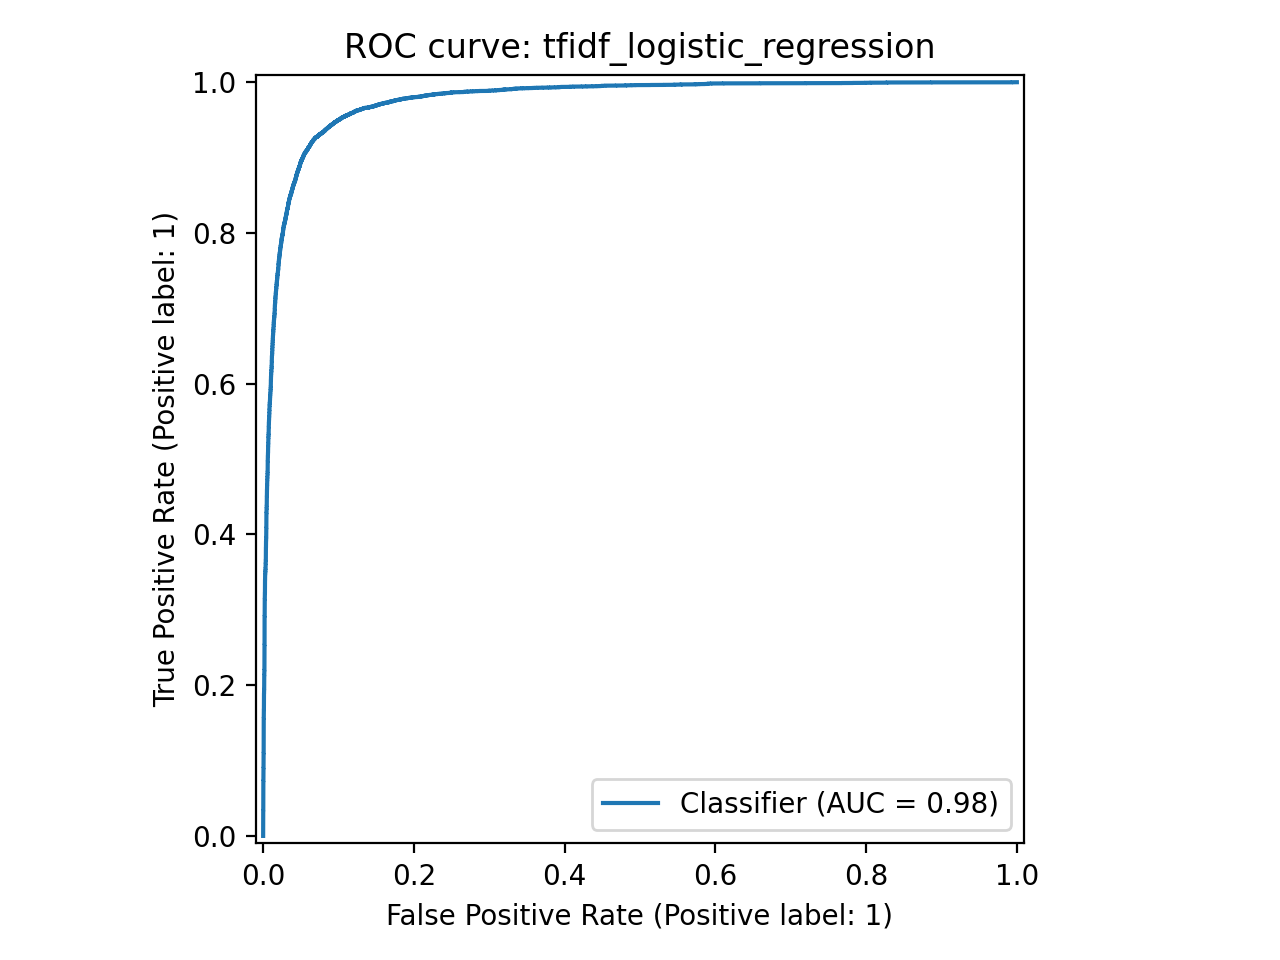
\includegraphics[width=0.72\linewidth]{figures/roc_curve_best_model.png}
\caption{\textbf{Internal test ROC curve for the validation-selected model.} The selected model was TF-IDF logistic regression.}
\label{fig:roc}
\end{figure}

\begin{figure}[!ht]
\centering
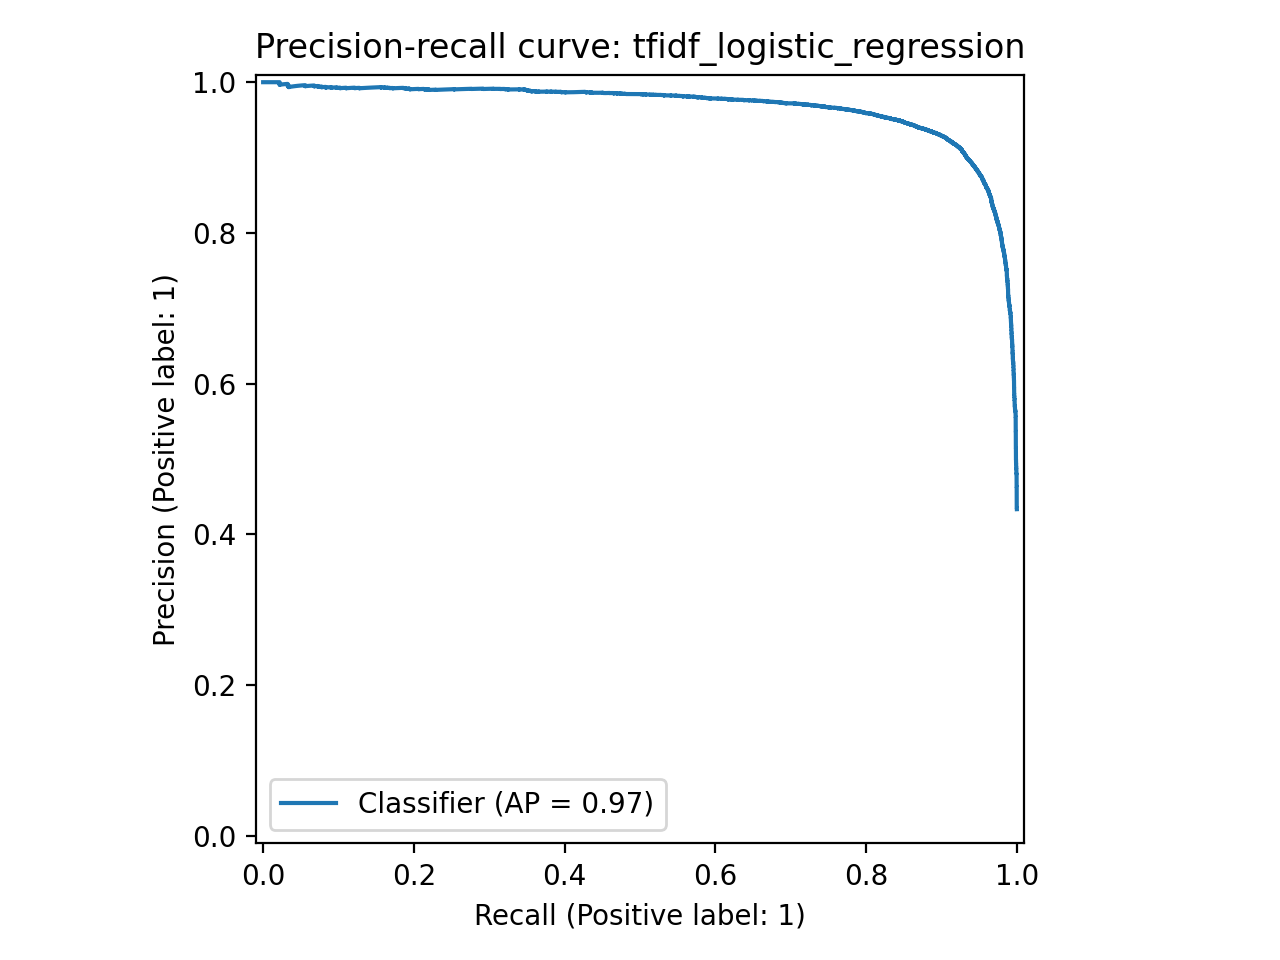
\includegraphics[width=0.72\linewidth]{figures/pr_curve_best_model.png}
\caption{\textbf{Internal test precision-recall curve for the validation-selected model.}}
\label{fig:pr}
\end{figure}

\begin{figure}[!ht]
\centering
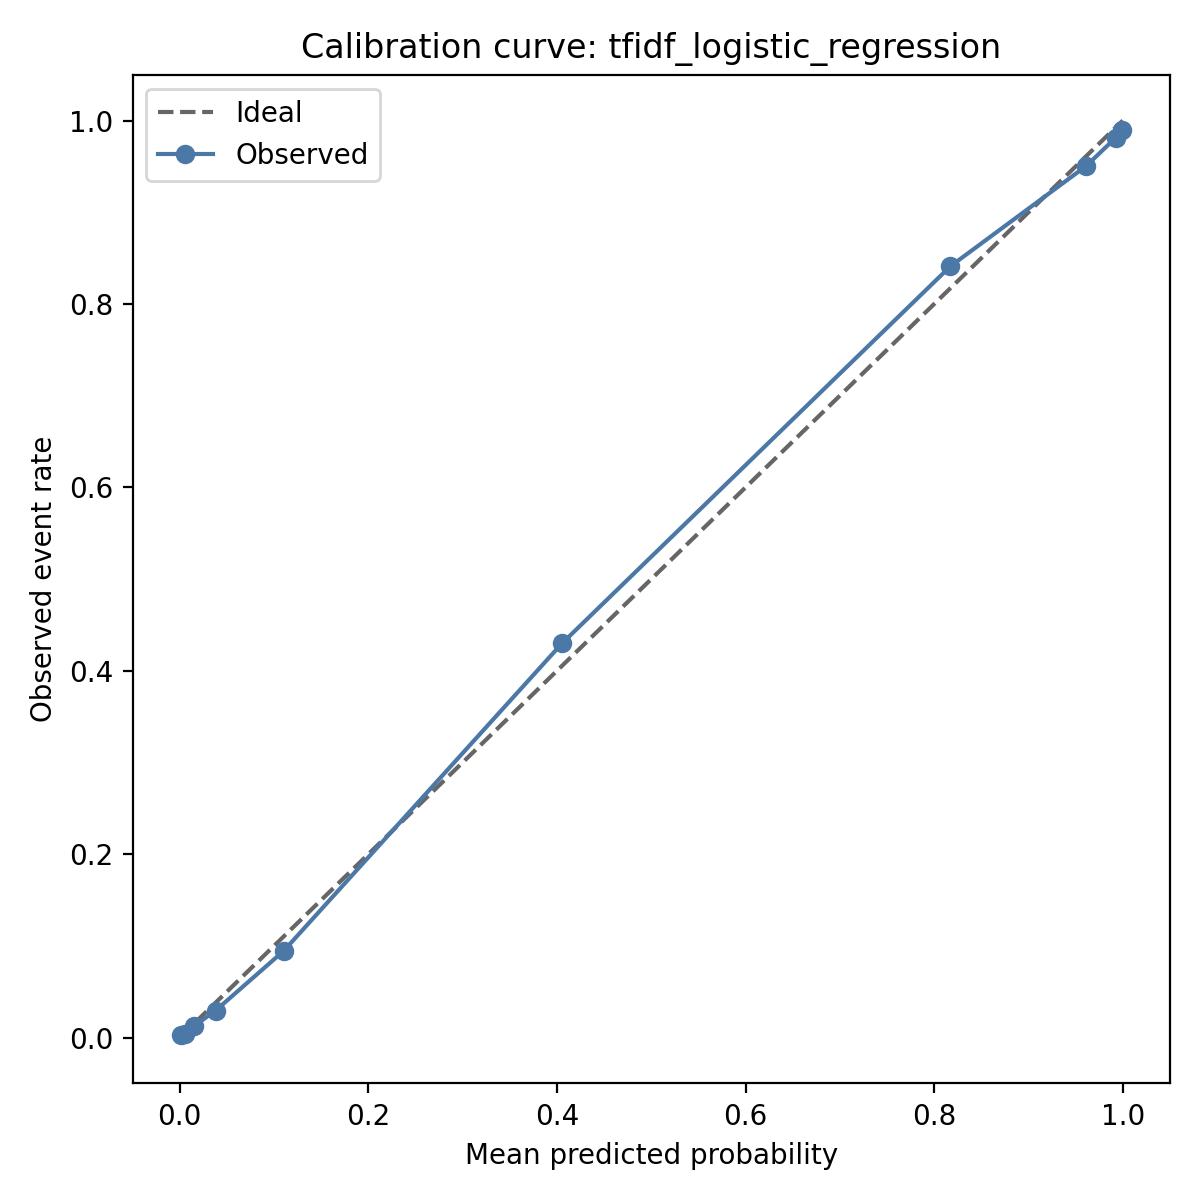
\includegraphics[width=0.72\linewidth]{figures/calibration_curve_best_model.png}
\caption{\textbf{Internal test calibration curve for the validation-selected model.}}
\label{fig:calibration}
\end{figure}

\begin{figure}[!ht]
\centering
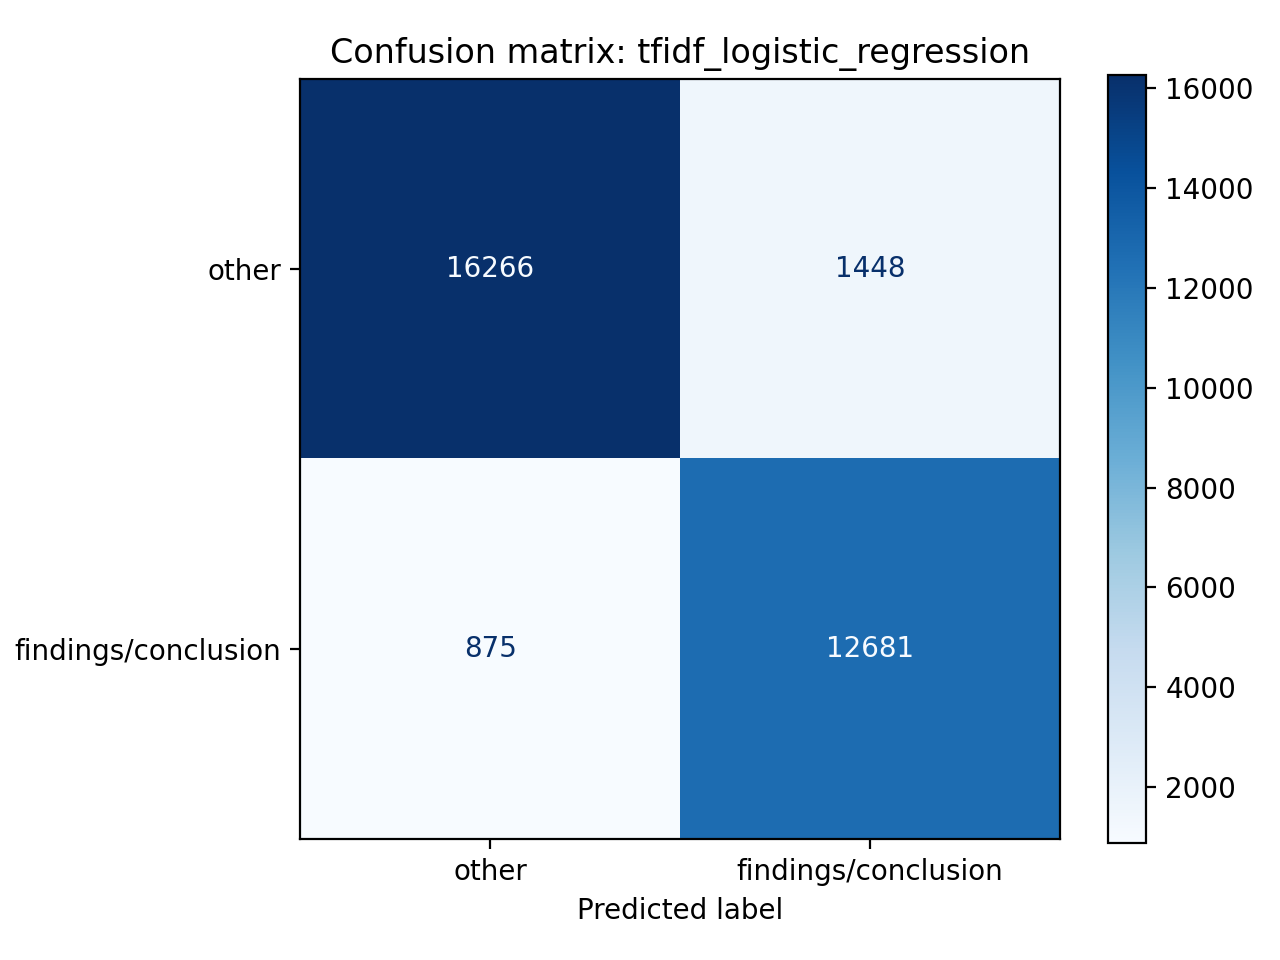
\includegraphics[width=0.72\linewidth]{figures/confusion_matrix_best_model.png}
\caption{\textbf{Internal test confusion matrix for the validation-selected model.}}
\label{fig:confusion}
\end{figure}

\begin{figure}[!ht]
\centering
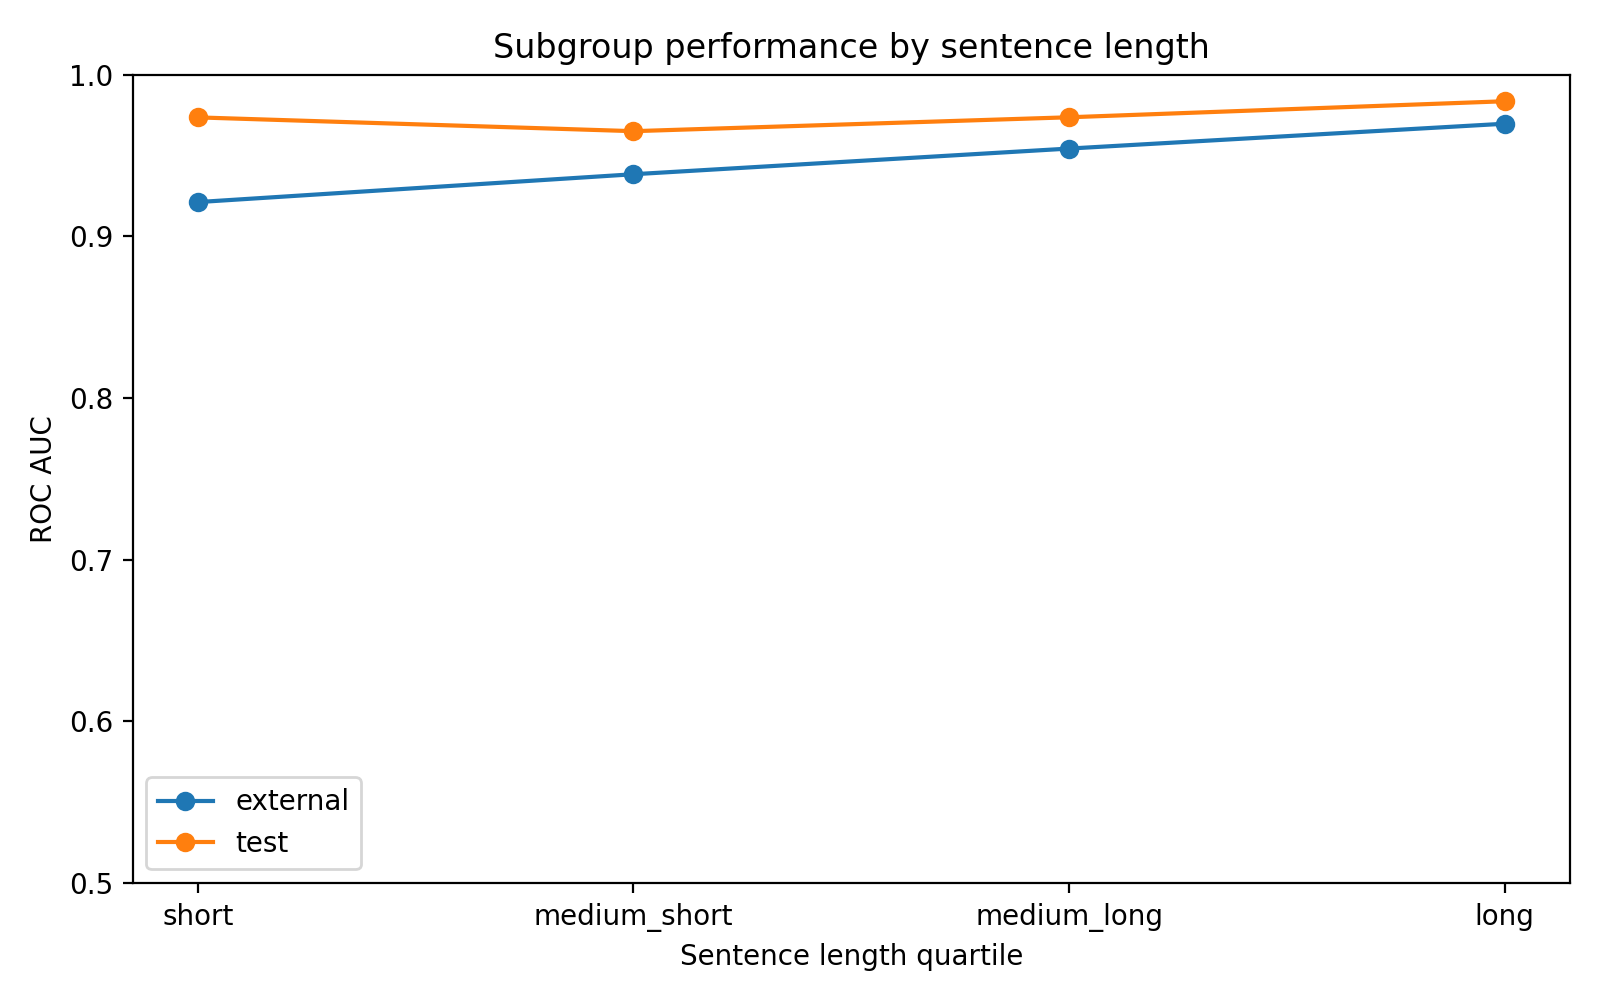
\includegraphics[width=0.72\linewidth]{figures/subgroup_performance.png}
\caption{\textbf{Sentence-length subgroup performance.} Subgroups are descriptive length quartiles.}
\label{fig:subgroup}
\end{figure}
